\subsection{Registered dose transfer and prospective precision design}
A metadata-qualified extension uses 24 lexicographically selected compounds at four exact doses across A549, K562 and MCF7, at 24 hours. All outcomes are exposed development. An initial plate-specific run stopped on missingness before scoring; an explicit amendment pools matched-control-subtracted plate means within each line. Four global dose holdouts retain 72 profiles each and 512 control-selected genes. Nested source-dose selection compares zero, mean and nearest-dose references with 30 fixed ridge/kernel curves. Query controls may select the gene panel; held-dose effects never enter fitting, scaling, selection or pretraining \citep{opaldose2026}.
\begin{center}\small\begin{tabular}{rrrrr}\toprule
Dose (nM) & Reference MSE & Smooth MSE & Gain & Paired reduction interval\\\midrule
10 & 0.037674 & 0.050863 & -35.01\% & [-0.022821, -0.000754]\\
100 & 0.028909 & 0.026544 & 8.18\% & [0.000883, 0.004364]\\
1000 & 0.052405 & 0.028459 & 45.69\% & [0.005018, 0.047922]\\
10000 & 0.060991 & 0.068715 & -12.66\% & [-0.021095, 0.009771]\\
\bottomrule\end{tabular}\end{center}
Both interpolation doses pass the 5\% development screen with positive conditional compound-bootstrap lower bounds; both extrapolation doses fail. Fitting takes 1.78 CPU seconds with final working set 201.5 MB. Bootstrap intervals condition on shared controls and three cell lines, excluding biological and selection uncertainty. An experimental known-compound/known-state interpolation reference preserves the selected source-dose curves and rejects extrapolation, unknown identities and endpoint mismatches; restored scored predictions agree within 0. No pair/context or chemical identity transfer claim follows.
\begin{figure}[ht]\centering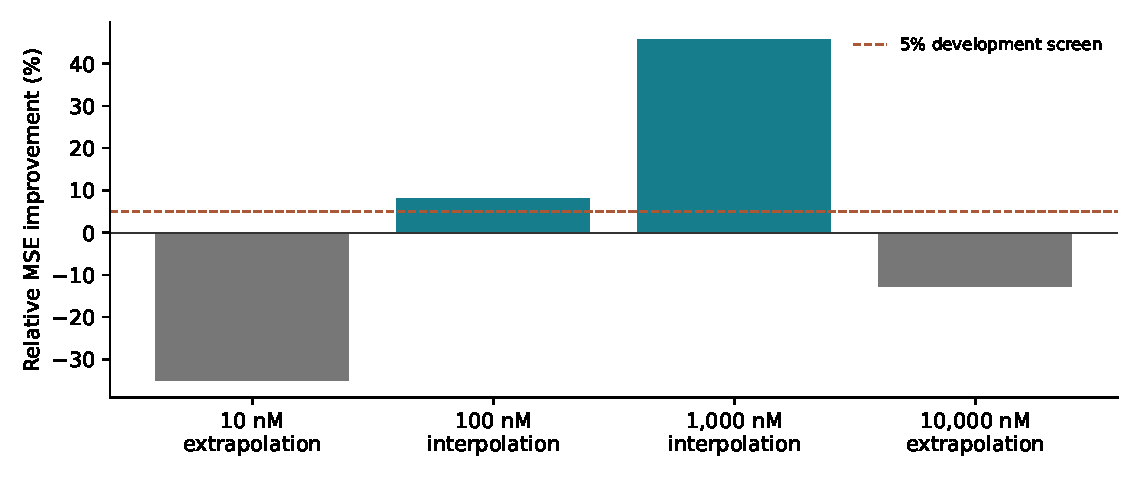
\includegraphics[width=.78\linewidth]{evidence/dose_results.pdf}\caption{Source-selected smooth dose curves improve interior doses and fail extrapolation on exposed sci-Plex development.}\end{figure}
A separate prospective sensitivity calculation evaluates 320 hypothetical designs with 2,000 Gaussian draws each. Crossed state, culture, target, pair and shared-control effects remain correlated; cell noise alone decreases with cell count. Assumed variance is not estimated from technical halves. The known-variance lower bound is optimistic and does not establish a powered sample size. Four development states with three independently initiated cultures per state form a variance pilot; broad transfer requires multiple sealed states and globally held pairs. The pilot must estimate biological covariance and mean precision before an empirical power calculation.
\begin{figure}[ht]\centering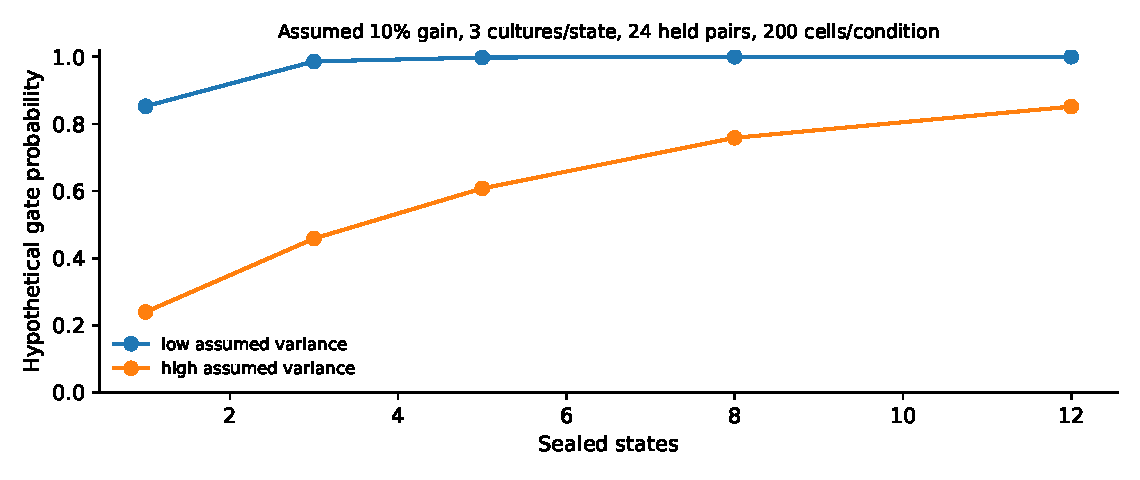
\includegraphics[width=.78\linewidth]{evidence/precision_sensitivity.pdf}\caption{Hypothetical design sensitivity under declared low and high variance assumptions. These are simulated design probabilities, not empirical confidence in Opal.}\end{figure}
